%! Suppress = LineBreak
\documentclass{acl2020}
\graphicspath{ {./fig/} }

%\aclfinalcopy % Uncomment this line for the final submission
%\def\aclpaperid{***} %  Enter the acl Paper ID here

\title{Targeted Sentiment Analysis}

\author{Maria Singstad Paulsen \\
  Department of Informatics – University of Oslo\\
  \texttt{marispau@ifi.uio.no}}
  
\date{}

\begin{document}
\maketitle

\begin{abstract}

\end{abstract}

\section{Motivation}
\label{sec:motivation}

In this paper, there are two overarching topics that will be presented to the reader. Though they differ in many ways, they are not entirely unrelated. The experiments cover analysis and evaluation of using different pre-trained word embeddings, from generalised to domain-specific, for fine-grained sentiment analysis, The other main topic has partially come as a by-product of the first, and concerns the choiced made with regards to the underlying codebase. Code that can be reused and distributed freely is a valuable tool and contribution to the open-source community. I have worked with this in mind, and focused equally much on reusability as reproducibility.

\section{Introduction}
\label{sec:intro}

Within the field of sentiment classification, there are several flavours — so to speak — to pick and choose from.
At the core of any sentiment analysis task, is the sentiment itself. In its most simplistic form, it often boils down to a binary classification task, where the goal then becomes to predict one of two polar opposites. This can be expanded to not only cover the sentiment itself, but also the target thereof, and further to include a scale rather than polar opposites. The dataset used in this work is annotated with targets, but sentiments are polar and not on a scale.


\section{The NoReC$_{\mathit{fine}}$ dataset}
\label{sec:data}

The dataset used in this work, NoReC$_{\mathit{fine}}$, is a recent addition to the collection of datasets for Norwegian, and the first one annotated for fine-grained sentiment analysis.
This dataset and annotation efforts are described in detail by \citet{norec_fine} in \emph{A Fine-Grained Sentiment Dataset for Norwegian}, while the underlying corpus is described in \emph{NoReC: The Norwegian Review Corpus}~\citep{velldal-etal-2018-norec}.  \\

\medskip
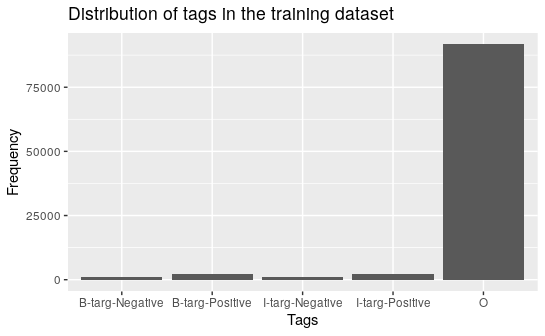
\includegraphics[width=220px]{fig/tag_frequencies_train.png}

\section{Related work}
\label{sec:background}

Mention NoReC parsing (ltgoslo github + article).
Refer to Learning Word Vectors for 157 Languages \citep{grave-etal-2018-learning}
Refer to Evaluating Semantic Vectors for Norwegian (thesis)
Refer to Enriching Word Vectors with Subword Information \citep{bojanowski-etal-2017-enriching}
Refer to Bag of Tricks for Efficient Text Classification \citep{joulin-etal-2017-bag}

\subsection{Code today only what you can decode tomorrow}
\label{subsec:baseline}

The codebase written for this work originally consisted of two separate packages. The one of which the BiLSTM belongs, is described in this section, and the other in the section that follows. The neural network was written using Google's TensorFlow 2.0 API. This in and of itself amassed a fair amount of work and, given that the provided pre-code was written using Facebook's PyTorch API, will be described in sufficient detail in this section.
The neural network consists of modules from the Keras functional API. The necessary building blocks required for a neural network bears some semblance to those of the {\small\verb|tf.keras.Sequential|} API. However, the functional API is more flexible, and can handle models with non-linear topology, models with shared layers, and models with multiple inputs or outputs~\citep{func-api}. For an in-depth presentation of the TensorFlow API and its open-source codebase,\citep{tensorflow2015-whitepaper}, refer to \emph{TensorFlow: A system for large-scale machine learning}.

For the purpose of learning how to string together the various pieces required for a neural network, the sequential API, available both in TensorFlow and PyTorch, is both sufficient and well-suited. However, as the architectures become more complex, the advanced user might start to feel bounded by constraints and the lack of flexibility.

User-friendliness and \emph{best practices} are key-terms in fields more closely related to software engineering than data science and and similar concepts  more often discussed in the field of software engineering, I would like to address it for the purpose of motivating the paths taken to conclude the work presented in this paper.

One could hardly argue with is a natural progression from the sequential way of building neural networks, through the modular way, and, if there is a need for it, on to a fully object-oriented way, where most modules are tailor-made for the job at hand.

One of the main reasons why I chose to work with TensorFlow rather than PyTorch, was


\subsection{Reproducibility}
\label{subsec:reproducability}

An important aspect of conducting any form of research, is that of reproducibility. With respect to this project in particular, one of the challenges that arose was how to prepare the data in such a way that it was suited as input to a recurrent neural network, yet also maintaining the requirement for reproducible results. Accompanying this project's proposal, was code for a baseline model and various evaluation metrics. However, as this was written using the PyTorch API, most all the code forming the basis for this paper has been written from scratch. As a direct result of this, one major difference between the PyTorch and TensorFlow models, lies in the lack of padding on batch level in the latter. One option explored was that of using the Dataset pipeline, another was using custom generators. In the case of the former, there would be a need to pad both the training and development datasets to the same length. As for the latter, it is not suitable if the model is to be serialised and restored in a different setting at a later time. That is, to say the least, sub-optimal when reproducibility matters.

On the topic of serialising, one other significant issue was that of not being able to deserialise all of the word embeddings trained to use in this experiment. The embeddings were produced using the Gensim library, and tests were done for embeddings created in modules that was part of the same package as the neural network and the rest of the code, as well as a stand-alone package. It was in the case of the latter that deserialising with {\small\verb|pickle.load()|} became rather troublesome. Given the scope and allotted time, a satisfactory solution did not seem feasible.

Whenever a seed was either suggested or required, the same seed was used troughout. In addition, a global seed was set through the TensorFlow API rather than using that of the Numpy API. The latter offers a well-known and much used module, {\small\verb|numpy.random|}, though it is recommended that the new BitGenerator~\footnote{https://numpy.org/doc/1.18/reference/random/index.html} be used instead. So as to not inadvertedly cause any incompatibility issues, whenever possible, the seeds have been set through the TensorFlow API. As part of writing the codebase,


\section{Beyond the Baseline: Taking The Modular Approach}
\label{sec:codebase}

This work is in its entirety based on but a single architecture. As was mentioned briefly in section~\ref{sec:motivation}, one of the goals has been to not only conduct experiments and report the findings, but also to be able to contribute towards the collective body of work that is open-source.

The architecture of the baseline model is a bi-directional long short-term memory recurrent neural network, BiLSTM for short.
Much like the RNN relaxes the Markov assumption and allows looking arbitrarily back into the past, the bi-directional RNN relaxes the fixed window size assumption, allowing to look arbitrarily far at both the past and the future within the sequence~\citep{neural-nlp}.

The intention lay in the wish for a reusable codebase that would lend itself to other projects in the future, as well as perhaps others wanting to train word embeddings for their own projects. The small module provides the end-user with a quick and easy way of training word embeddings that can be used with the neural network.

\section{From generalised to domain-specific embeddings}
\label{sec:embeddings}

There is a plethora of different word embeddings to choose from, including embeddings trained for Norwegian. In my experiements, I chose to focus on embeddings carrying subword information, due to the nature of the task at hand, and did only include embeddings where the full word form has been kept intact. The baseline embeddings model was trained on Common Crawl using fastText~\citep{grave-etal-2018-learning}. The model was trained using CBoW with position-weights, in dimensions 300, with character n-grams of length 5, a window of size 5 and 10 negatives. As mentioned in section \section{data}, NoReC$_{fine}$ is a dataset based on a subset of the larger NoReC corpus. There is a decent amount of pre-trained word embeddings available for Norwegian distributed through the NLPL website~\footnote{http://vectors.nlpl.eu/}, but none of which has been trained on the NoReC corpus.

I decided to use the fastText Common Crawl embeddings as the embeddings baseline for two reasons. One came down to the selection of embeddings in the NLPL repository, and the other  because I wanted to train domain-specific ones. In order to be able to compare and contrast, it seemed reasonable to start with one that I suspected might differ somewhat from the rest. As it turned out, this was not really the case after all.

In her thesis, \emph{Evaluating Semantic Vectors for Norwegian}, \citet{StadsnesCathrine2018ESVf} trains, evaluates and presents results for several of the word embeddings now found in the NLPL repository. Based on her findings, I decided to focus my attention on embeddings trained on the Norwegian Newspaper Corpus (NNC) and The Norwegian Web as Corpus (NoWaC), and, for the most part, excluded those trained on the NBDigital Corpus (NBDigita). The embeddings trained on all three, did not perform well, and not better than any of the embeddings trained on either NNC or NoWaC alone, nor the NoReC embeddings.

\subsection{Training on the NoReC corpus}
\label{subsec:norec-emb}

All of the embeddings trained for this project used either fastText skipgram or fastText continuous bag-of-words. I used windows of size 5 and 10, a minimum word count of between 4 and 8 and dimensionalities 100 and 300. I trained embeddings on the NoReC train partition, a combination of the train and development partition~\footnote{These were not actually used, and so the results are not included in the findings.}, the Norwegian Dependency Treebank (NDT), and a combination of NoReC and NDT.

Sentences were parsed from CoNNL-U to a single sentence per line so as to comply with the {\small\verb|PathLineSentences|} class in the Gensim library, and was not pre-processed any further.


\section{Analysis}
\label{sec:error-analysis}

All things, and efforts, considered, there are disappointingly few results worth boasting about. The domain-specific embeddings ranked highest in terms of both binary and proportional scores, but this alone is not enough to base a conclusion on. As

\section{Conclusions and Outlook}
\label{sec:conclusion}

The embeddings trained on the NoReC corpus showed potential. However, being that they are domain-specific, it is not unlikely that it would be more beneficial to combine them with embeddings trained for other domains, either by training on a larger set of data, or tackle it whilst building the neural network. Fine-tuning the model would also be necessary in order to draw any conclusions.

\bibliographystyle{acl_natbib}
\bibliography{references,anthology,acl2020}

\appendix

\section{Appendices}
\label{sec:appendix}

\end{document}

% \begin{table}[ht]
% \caption{Multi-column table}
% \begin{center}
% \begin{tabular}{lcccccc}
%     \toprule &
%         \multicolumn{2}{c}{\textbf{Training}} &
%         \multicolumn{2}{c}{\textbf{Development}} &
%         \multicolumn{2}{c}{\textbf{Evaluation}} \\
%     \midrule \textbf{Polarity} &
%         Pos & Neg & Pos & Neg & Pos & Neg \\
%     \midrule \textbf{B or I} &
%         200 & 180 & 70 & 60 & 50 & 60 \\
%         \textbf{B-targ} & \multicolumn{2}{c}{380} &
%         \multicolumn{2}{c}{130} &
%         \multicolumn{2}{c}{110} \\
%         \textbf{I-targ} & \multicolumn{2}{c}{5000} &
%         \multicolumn{2}{c}{1150} &
%         \multicolumn{2}{c}{1100} \\
%         \textbf{Total} & \multicolumn{2}{c}{5000} &
%         \multicolumn{2}{c}{1150} &
%         \multicolumn{2}{c}{1100} \\
%     \bottomrule
% \end{tabular}
% \end{center}
% \label{tab:multicol}
% \end{table}